\begin{frame}
    \frametitle{M\'etodo de vol\'umenes finitos}
    \framesubtitle{Errores inducidos por la malla}

    \begin{center}
      Adem\'as de los errores de truncamiento presentes por considerar discretizaciones espaciales y temporales de segundo orden, surgen t\'erminos de error debido a la \textcolor{red}{elecci\'on de la malla. }
      \end{center}

    \begin{itemize}

    \item \textbf{No ortogonalidad}: si no se considera la componente no ortogonal del t\'ermino difusivo (para acotar la soluci\'on), la discretizaci\'on del t\'ermino difusivo suma un t\'ermino de error
      $$ E_d = \sum_f \bs{S} \cdot \left [ (\rho \bs{U})_f \bs{k} (\nabla \phi)_f  \right ]  = \nabla \cdot ( (\rho \bs{U})_f \bs{k} \cdot \nabla \phi) = \nabla \cdot (\Gamma_D \cdot \nabla \phi)$$
      La magnitud del error depende del \'angulo de no ortogonalidad y de la aproximaci\'on. Es m\'inimo para la correcci\'on m\'inima.
      
      
    \end{itemize}

\end{frame}


\begin{frame}
    \frametitle{M\'etodo de vol\'umenes finitos}
    \framesubtitle{Errores inducidos por la malla}

    \begin{itemize}

    \item \textbf{Oblicuidad (skewness)}:

      \begin{columns}
      
      \column{0.4\textwidth}
      \begin{figure}[h]
        \begin{center}
          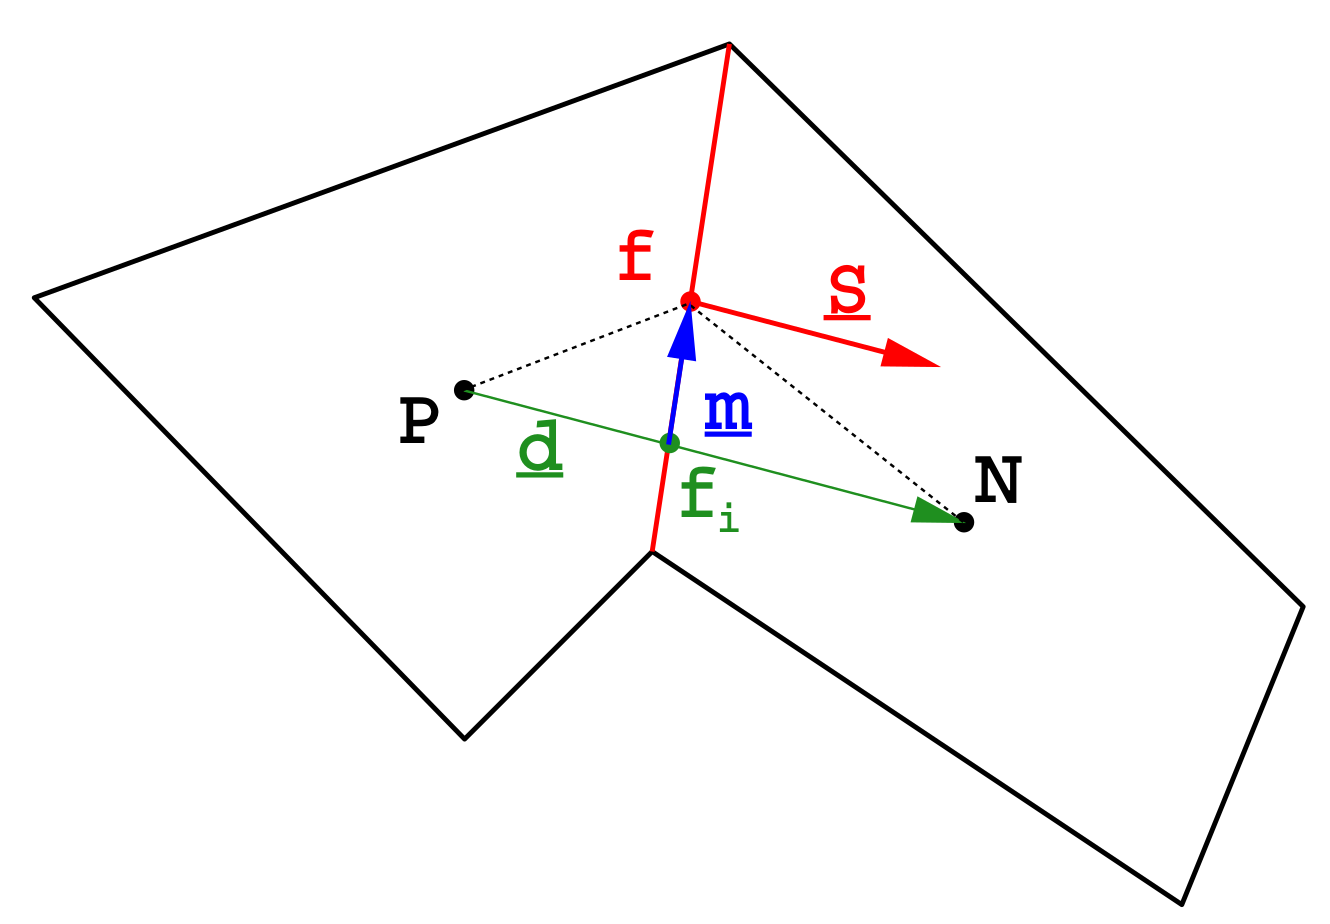
\includegraphics[width = \textwidth]{Imagenes/Skew}
        \end{center}
      \end{figure}

      
      \column{0.55\textwidth}
      \small
      El c\'alculo de integrales sobre las caras requiere el valor de la variable en el centro de la misma

      $$ \int_f d\bs{S} \phi = \bs{S} \phi_f $$

      Pero si $\phi_f$ se obtiene por interpolaci\'on lineal usando $P$ y $N$, en realidad se calcula $\phi$ en el punto $f_i$

      \end{columns}

      \vspace{0.5cm}
      \small
      El error puede estimarse como
      $$ E_s = \sum_f \bs{S} \cdot (\rho \bs{U} \delta \phi)_f = \sum_f \bs{S} \cdot \left [ (\rho \bs{U} )_f \bs{m} \cdot (\nabla \phi)_f \right ]$$
      con $\bs{m} = \bs{x}_f - \bs{x}_{f_i} $
      
      
      
    \end{itemize}

\end{frame}
